
\documentclass[11pt]{exam} % https://www.ctan.org/pkg/exam?lang=en

\usepackage[lmargin=1.in,rmargin=1.in,tmargin=1.in,bmargin=1in]{geometry}
\usepackage{setspace}
\usepackage[pdftex]{graphicx}
\usepackage{titling}
\usepackage[
	pdfauthor={Brian Weinstein},
	pdftitle={Homework 4},
	bookmarks=true,
	colorlinks=true,
	linkcolor=blue,
	urlcolor=blue,
	citecolor=blue,
	pdftex,
	linktocpage=true
	]{hyperref}
\usepackage[textsize=tiny]{todonotes}
\usepackage{float}
\setlength\parindent{0pt}
\usepackage{lipsum}
\usepackage{amsmath}
\usepackage{caption}


\qformat{\textbf{Problem \thequestion: \thequestiontitle}\quad \hfill}


\pagestyle{headandfoot}
\runningheadrule
\firstpageheader{}{}{}
\runningheader{\theauthor}{\thetitle}{\thedate}
\firstpagefooter{}{\thepage}{}
\runningfooter{}{\thepage}{}


\usepackage{xcolor}
\usepackage{adjustbox}
\usepackage{verbatim}
\definecolor{shadecolor}{rgb}{.9, .9, .9}

\newenvironment{code}%
   {\par\noindent\adjustbox{margin=1ex,bgcolor=shadecolor,margin=0ex \medskipamount}\bgroup\minipage\linewidth\verbatim}%
   {\endverbatim\endminipage\egroup}

\newenvironment{codeSmall}%
   {\par\noindent\adjustbox{margin=1ex,bgcolor=shadecolor,margin=0ex \medskipamount}\bgroup\minipage\linewidth\verbatim\footnotesize}%
   {\endverbatim\endminipage\egroup}

\newcommand{\ramsey}{\href{http://www.statisticalsleuth.com/}{Ramsey }}



\begin{document}


\title{STAT W4201 001, Homework 4}
\author{Brian Weinstein (bmw2148)}
\date{Feb 24, 2016}
\maketitle

Code is attached here and also posted at \href{https://github.com/BrianWeinstein/advanced-data-analysis}{https://github.com/BrianWeinstein/advanced-data-analysis}. Where relevant, code snippets and output are are included in-line.

\begin{questions}



\titledquestion{\ramsey 5.23}

The data provides overwhelming evidence that the mean oxygen isotopic composition in the 12 bone samples are different (a p-value of $9.7\times 10^{-7}$ from a one-way analysis of variance (ANOVA) F-test).

The ANOVA table testing for a difference in mean oxygen isotopic composition is shown below, and a boxplot of oxygen composition for each bone is shown in Figure \ref{fig:1}.

\begin{center}
  \begin{tabular}{ l c c c c c}
    Source of Variation & Sum of Squares & d.f. & Mean Square & F-Statistic & p-Value \\ \hline \hline
    Between Groups & 6.0675 & 11 & 0.55159 & 7.4268 & $9.73\times 10^{-7}$ \\
    Within Groups & 2.9708 & 40 & 0.07427 & & \\ \hline
    Total & 9.0383 & 51 & & &
  \end{tabular}
\end{center}
\quad \\

\begin{figure}[!h]
	\centering
	\captionsetup{width=0.8\textwidth}
	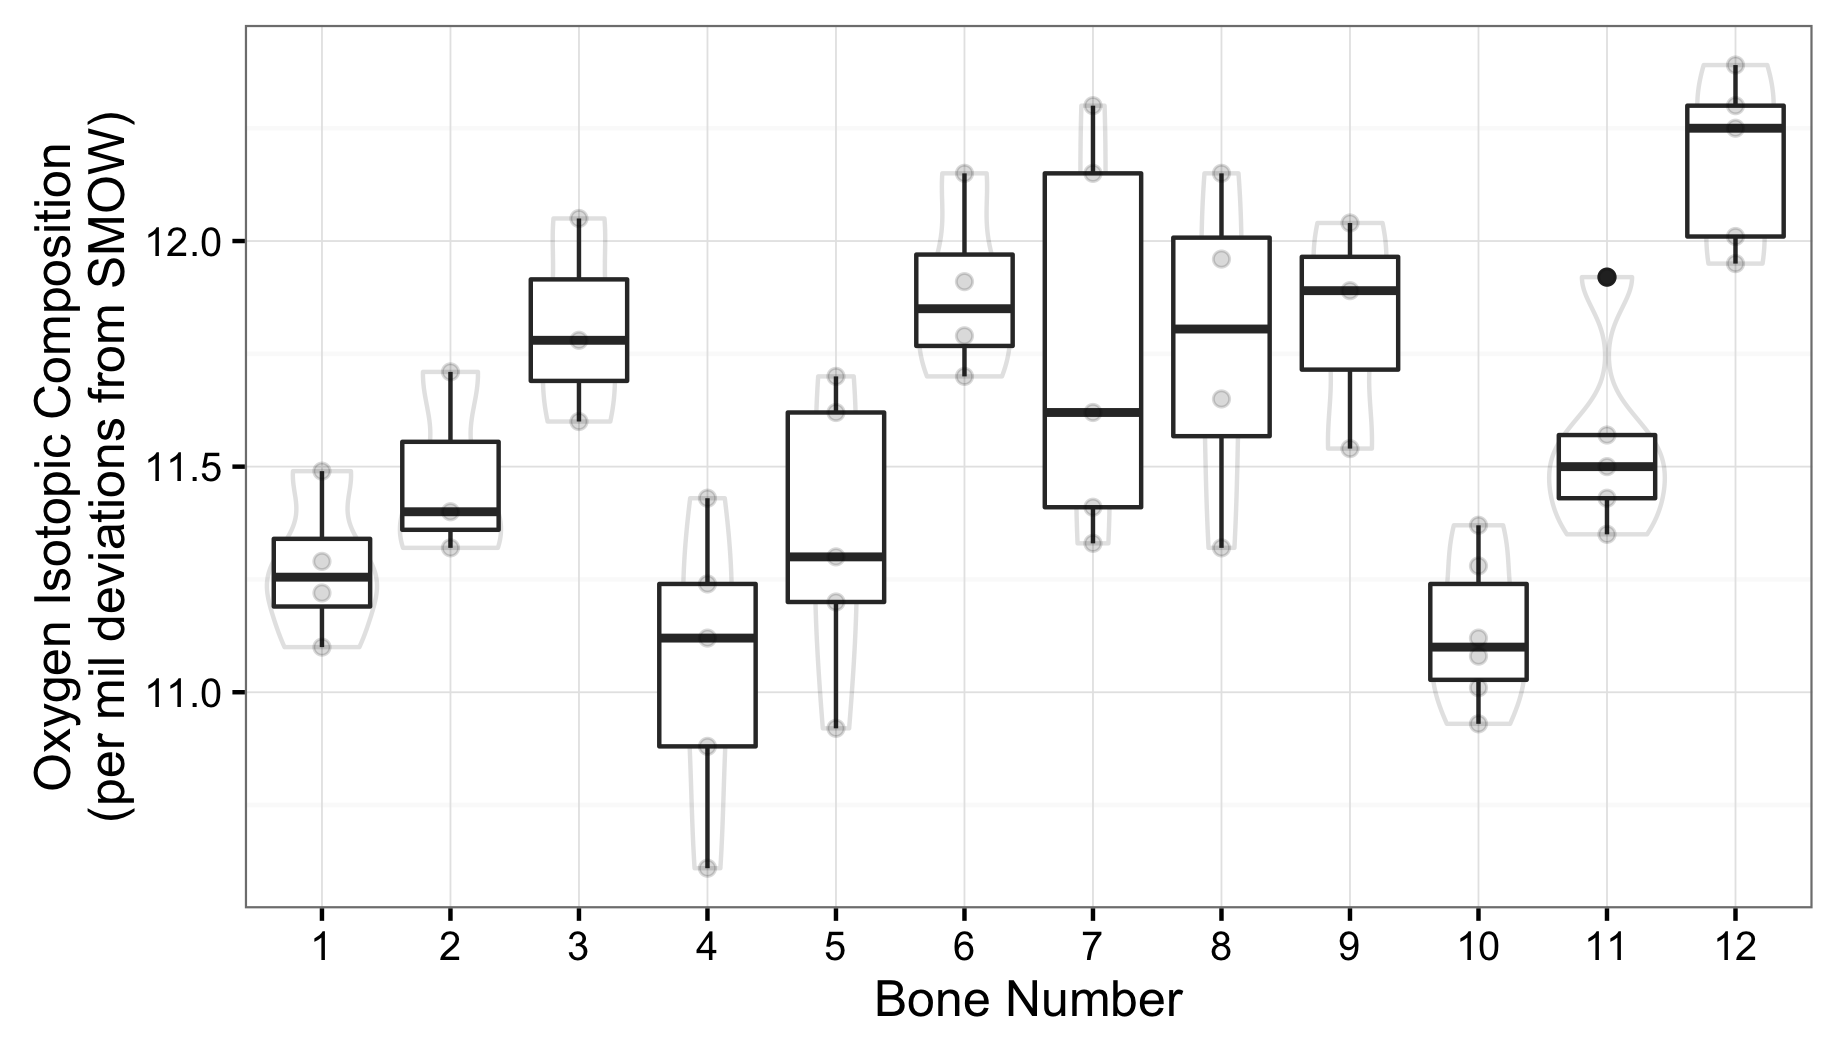
\includegraphics[width=4.25in]{1.png}
	\caption{Oxygen Isotopic Composition (per mil deviations from SMOW) for twelve bones of a single Tyrannosaurus rex specimen.}
	\label{fig:1}
\end{figure}

\pagebreak

\titledquestion{\ramsey 5.25}

\begin{parts}
\setlength{\parindent}{1em}

\part \textit{How strong is the evidence that at least one of the five population distributions (corresponding to the different years of education) is different from the others?}

Figure \ref{fig:2a} shows the distribution of income for 5 different ``years of education'' groupings. The boxplots show (1) the presence of severe outliers, and (2) that the group standard deviations increase as the years of education increases.

\begin{figure}[!h]
	\centering
	\captionsetup{width=0.8\textwidth}
	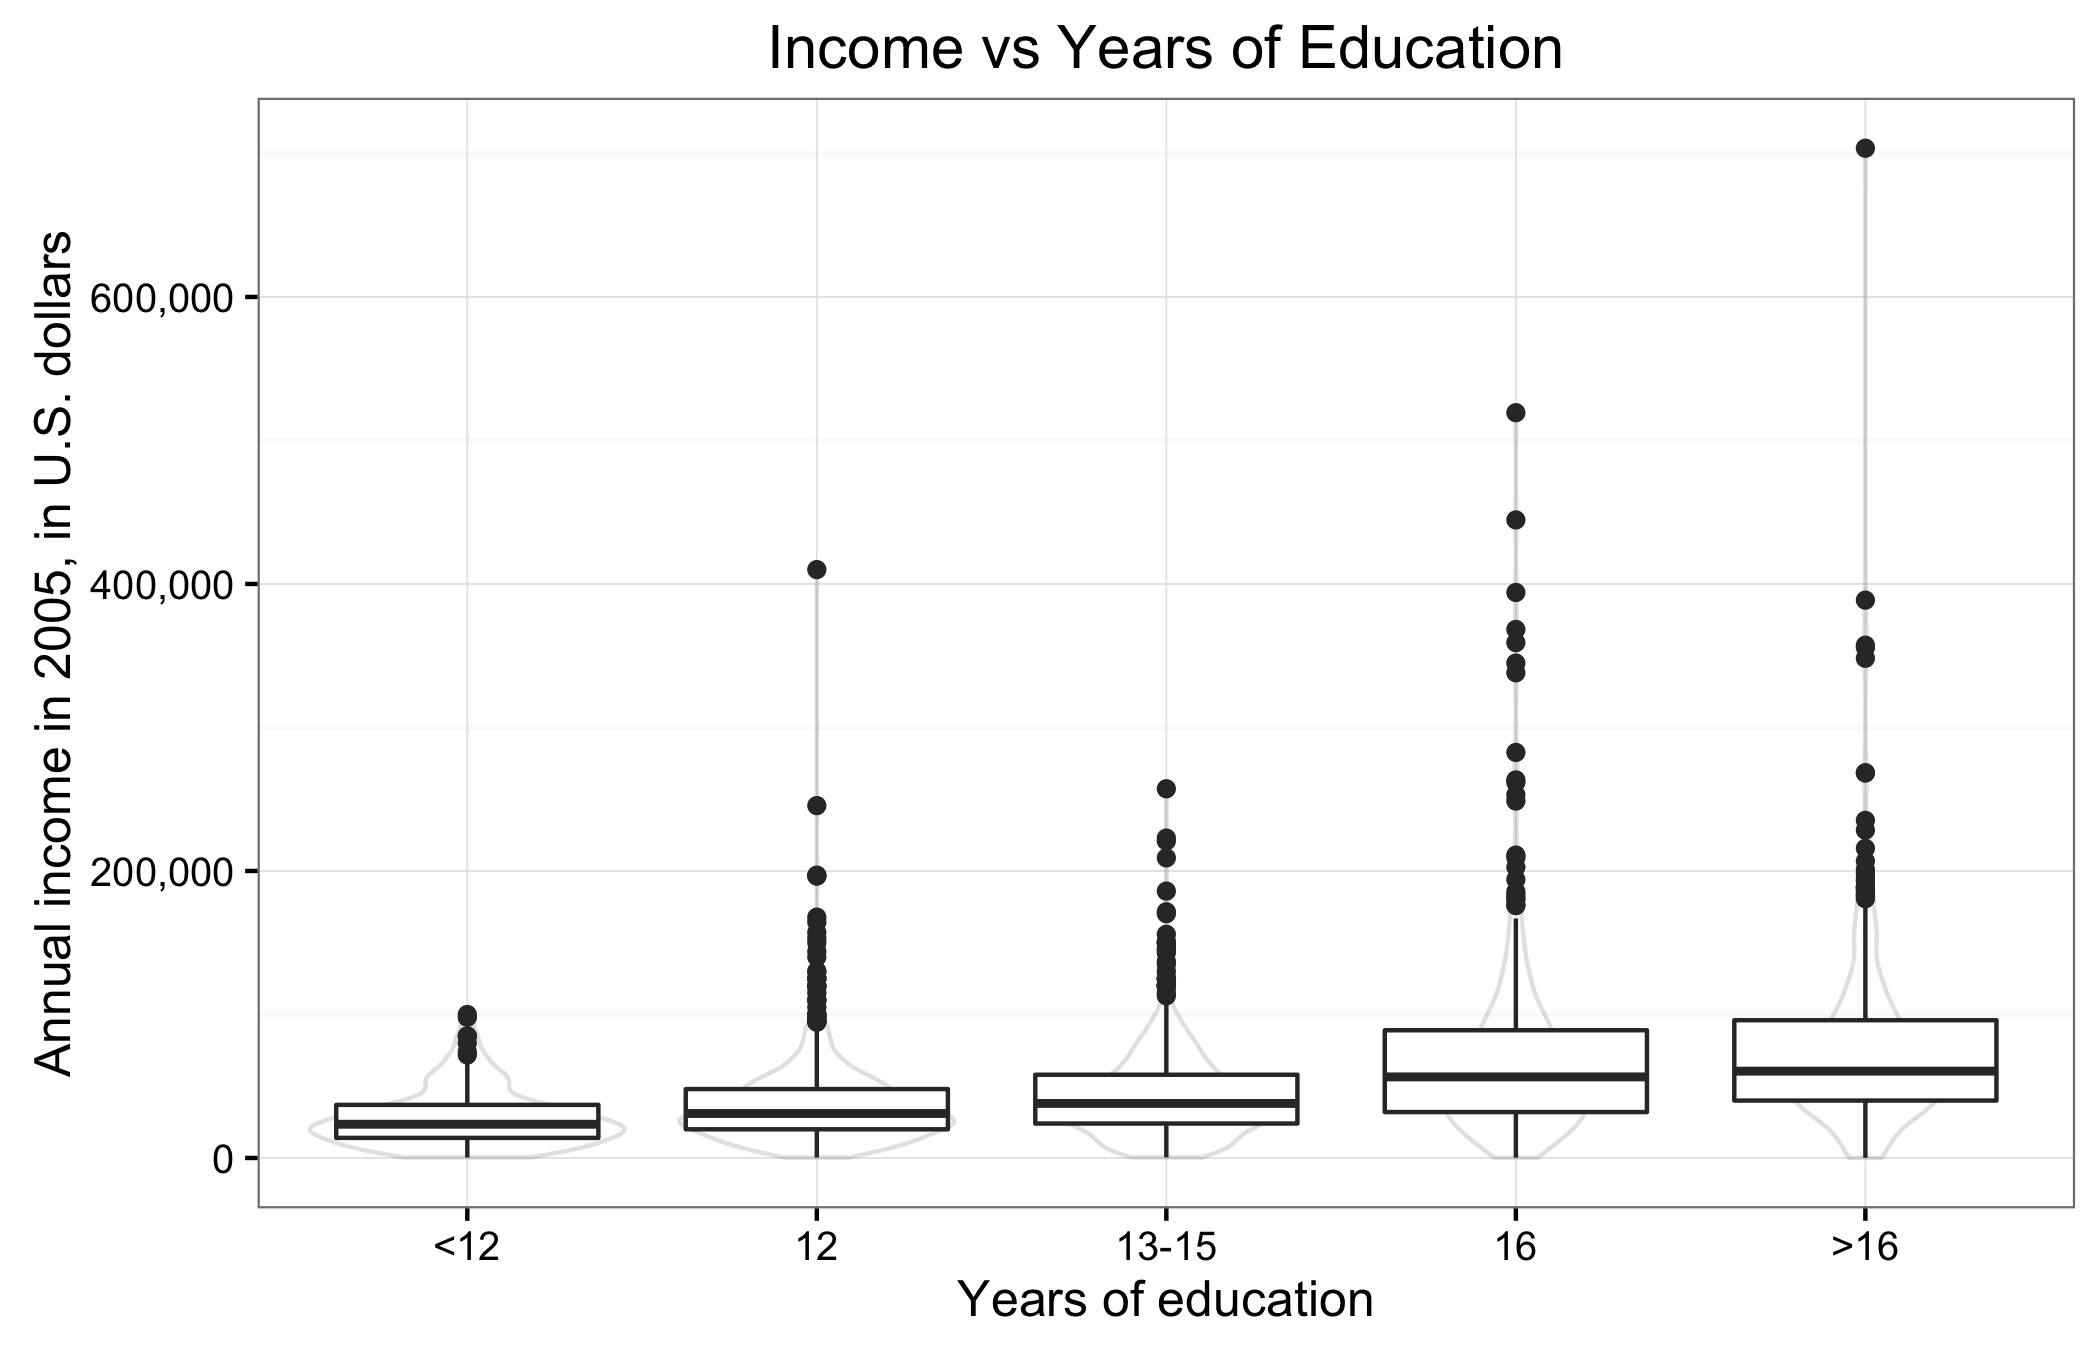
\includegraphics[width=4.25in]{2a.png}
	\caption{Income vs Years of Education for 2,584 observations among 5 ``Years of Education'' groupings.}
	\label{fig:2a}
\end{figure}

Examining the dataset, we also see that the group sample sizes are different.

\begin{codeSmall}
> # check group sample sizes and standard deviations
> incomeEduData %>%
+   group_by(Educ) %>%
+   summarize(numObs=n(), mean=mean(Income2005),
+             median=median(Income2005), stdev=sd(Income2005))
Source: local data frame [5 x 5]

    Educ numObs     mean median    stdev
  (fctr)  (int)    (dbl)  (dbl)    (dbl)
1    <12    136 28301.45  23500 21021.90
2     12   1020 36864.90  31000 29369.73
3  13-15    648 44875.96  38000 33913.54
4     16    406 69996.97  56500 64256.80
5    >16    374 76855.46  60500 65428.29
\end{codeSmall}

The F-tests are not robust to a lack of equal standard deviations and are not resistant to severe outliers. Since the education groups with higher mean incomes also have higher spreads, this dataset is a good candidate for a log transformation.

On the log scale, there are fewer outliers (which are also less-severe) and the standard deviations are nearly equal, as shown in Figure \ref{fig:2b} and in the table below.

\begin{figure}[!h]
	\centering
	\captionsetup{width=0.8\textwidth}
	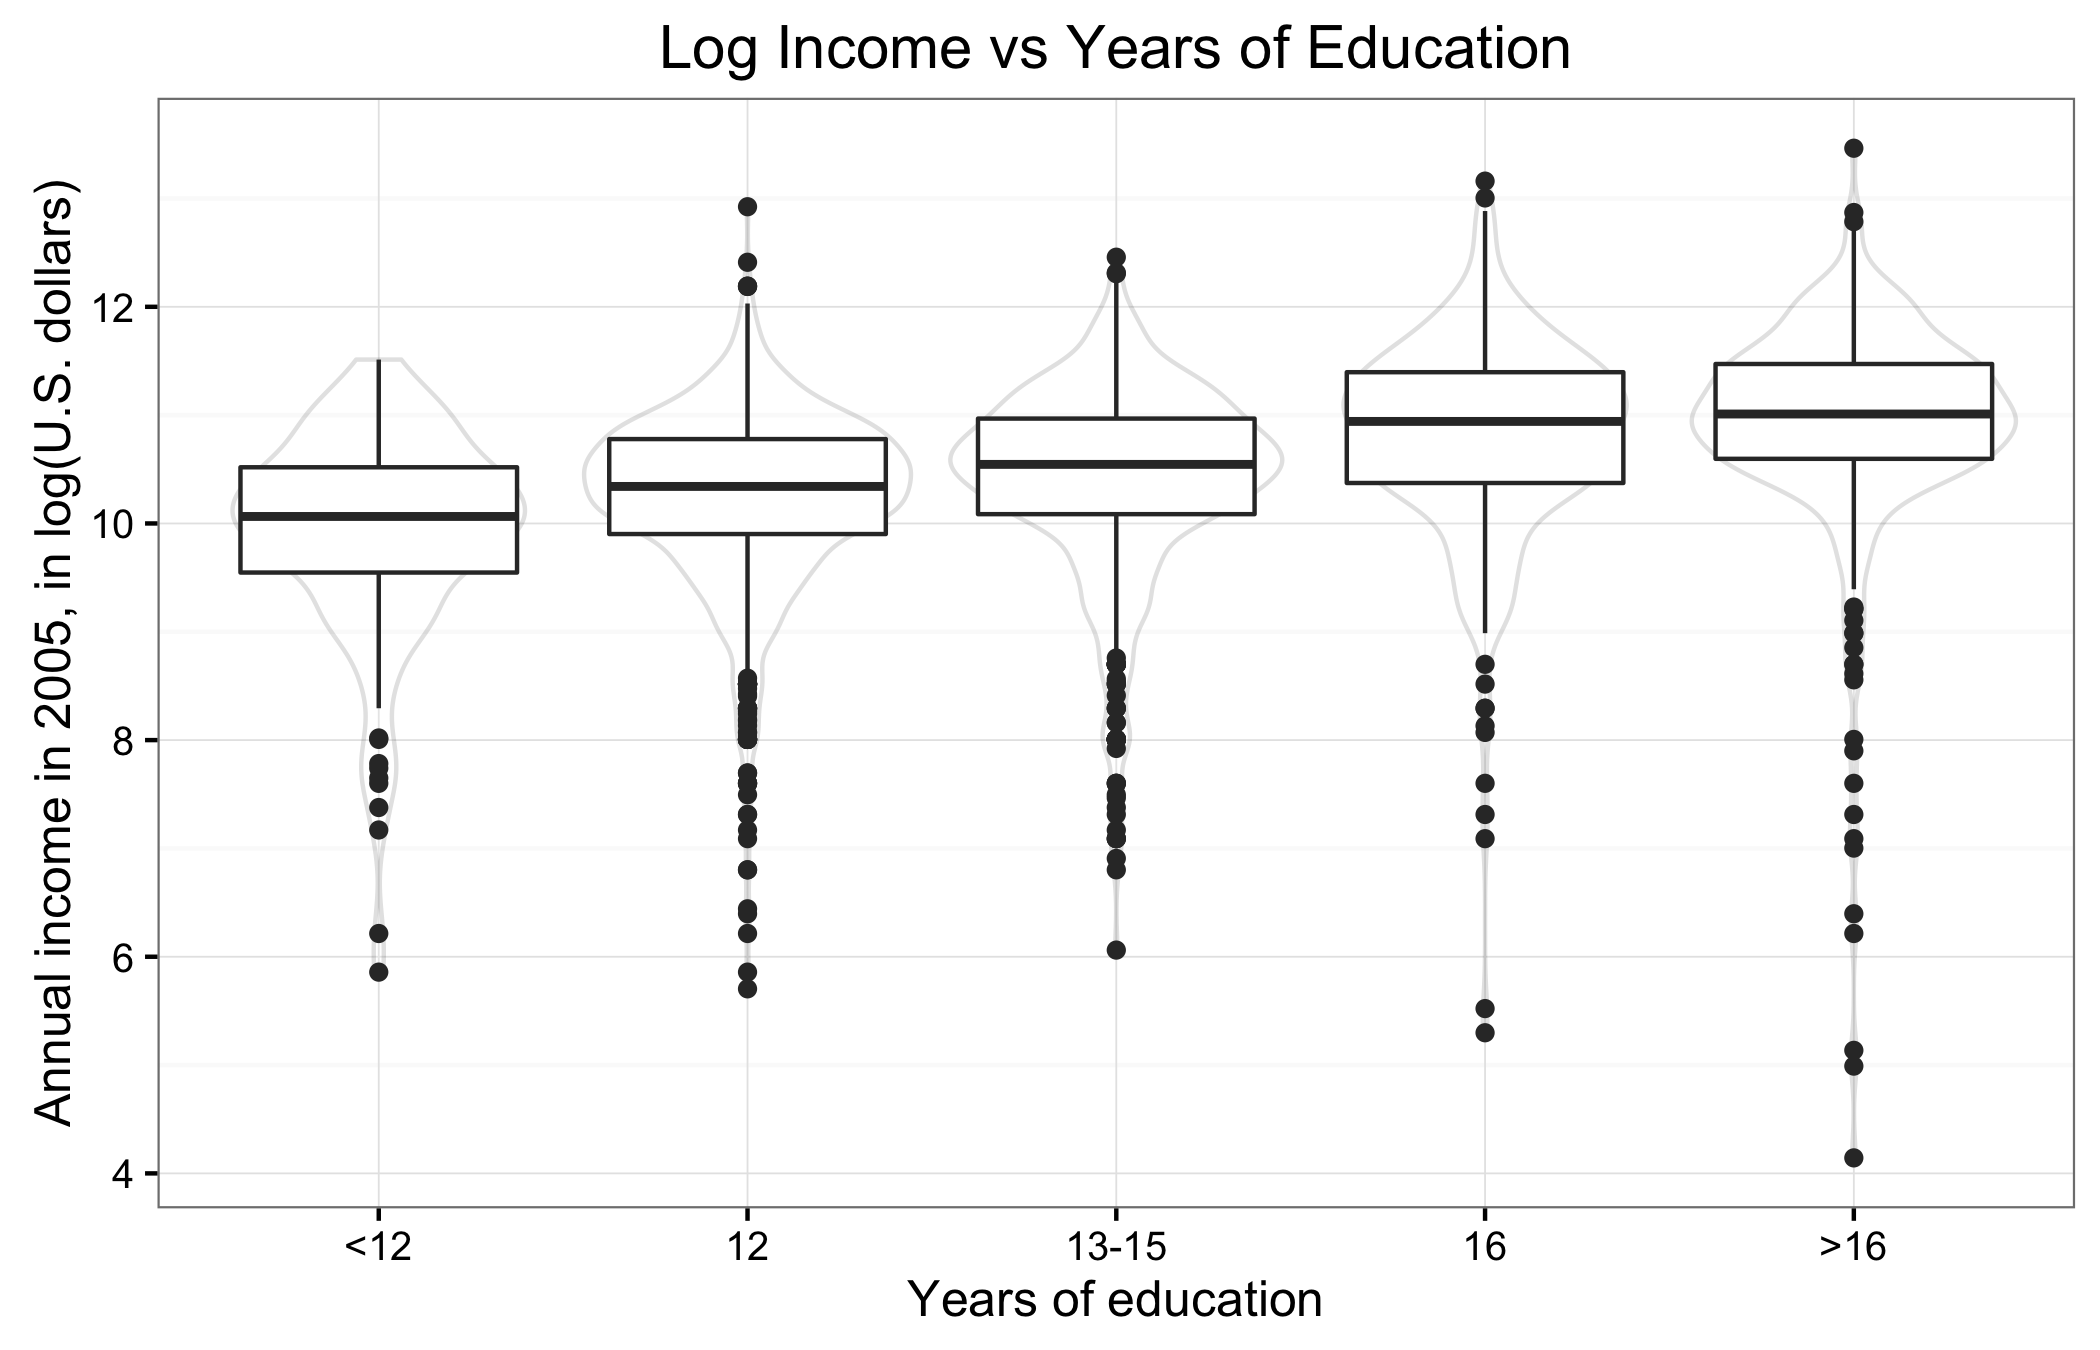
\includegraphics[width=4.25in]{2b.png}
	\caption{Log(Income) vs Years of Education for 2,584 observations among 5 ``Years of Education'' groupings.}
	\label{fig:2b}
\end{figure}

\begin{codeSmall}
> # check group sample sizes and standard deviations on log scale
> incomeEduData %>%
+   group_by(Educ) %>%
+   summarize(numObs=n(), mean=mean(LogIncome2005),
+             median=median(LogIncome2005), stdev=sd(LogIncome2005))
Source: local data frame [5 x 5]

    Educ numObs     mean   median     stdev
  (fctr)  (int)    (dbl)    (dbl)     (dbl)
1    <12    136  9.89934 10.06453 0.9988809
2     12   1020 10.22721 10.34174 0.8539854
3  13-15    648 10.39121 10.54534 0.9288173
4     16    406 10.79709 10.94196 0.9581051
5    >16    374 10.89790 11.01036 1.0665910
\end{codeSmall}

Performing the one-way ANOVA F-test on the log-transformed incomes we find overwhelming evidence that at least one of the five population distributions is different from the others. The ANOVA table is shown below.

\begin{center}
  \begin{tabular}{ l c c c c c}
    Source of Variation & Sum of Squares & d.f. & Mean Square & F-Statistic & p-Value \\ \hline \hline
    Between Groups & 217.65 & 4 & 54.413 & 62.87 & $2.2\times 10^{-16}$ \\
    Within Groups & 2232.12 & 2579 & 0.865 & & \\ \hline
    Total & 2449.774 & 2583 & & &
  \end{tabular}
\end{center}
\quad \\

Although it isn't entirely justified here (as per Display 3.6), when performing the ANOVA F-test on the dataset excluding outliers\footnote{Here, an outlier is defined as an observation more than 1.5 times the group interquartile range below the first quartile or above the third quartile.} we still find overwhelming evidence that at least one distribution is different from the others, so the results are not included here.



\part \textit{By how many dollars or by what percent does the mean or median for each of the last four categories exceed that of the next lowest category?}

The \texttt{CompareTwoEducGroups} function (see attached code for function definition) performs a two-sample t-test to test the hypothesis that the mean log income in the first specified ``Years of Education'' (YOE) group is greater than the mean log income in the second specified group. It outputs a one-sided p-value, an estimated value for the multiplicative treatment effect (in USD --- the original scale), and a 95\% confidence interval for the multiplicative treatment effect (also in USD).

\begin{subparts}
\setlength{\parindent}{1em}


\subpart \textbf{($>$16) vs (16)}

\begin{codeSmall}
> CompareTwoEducGroups(data_frame=incomeEduData, Educ_groups=c(">16", "16"))
 oneSidedPVal      estimate confInt_lower confInt_upper 
   0.08238005    1.10607335    0.95934487    1.27524345 
> CompareTwoEducGroups(data_frame=incomeEduDataExclOutliers, Educ_groups=c(">16", "16"))
 oneSidedPVal      estimate confInt_lower confInt_upper 
 3.968804e-05  1.224599e+00  1.107807e+00  1.353704e+00 
\end{codeSmall}

The data provides little evidence that the $>$16 YOE population earns a higher income than the 16 YOE population (one-sided p-value $0.08238$; two-sample t-test). A 95\% confidence interval for the number of times by which the $>$16 YOE income exceeds the 16 YEO income is $0.95934$ to $1.27524$ times. 

When excluding outliers, however, (see Figure \ref{fig:2c}) the data provides convincing evidence that the $>$16 YEO population earns a higher income than the 16 YOE population (one-sided p-value $3.97 \times 10^{-5}$; two-sample t-test). Income is estimated to be $1.22460$ times greater for the those with $>$16 YOE compared to those with 16 YOE, with a 95\% confidence interval of $1.10781$ to $1.35370$ times (i.e., an estimated 22\% increase; 95\% CI from 11\% to 35\%).

\begin{figure}[!h]
	\centering
	\captionsetup{width=0.8\textwidth}
	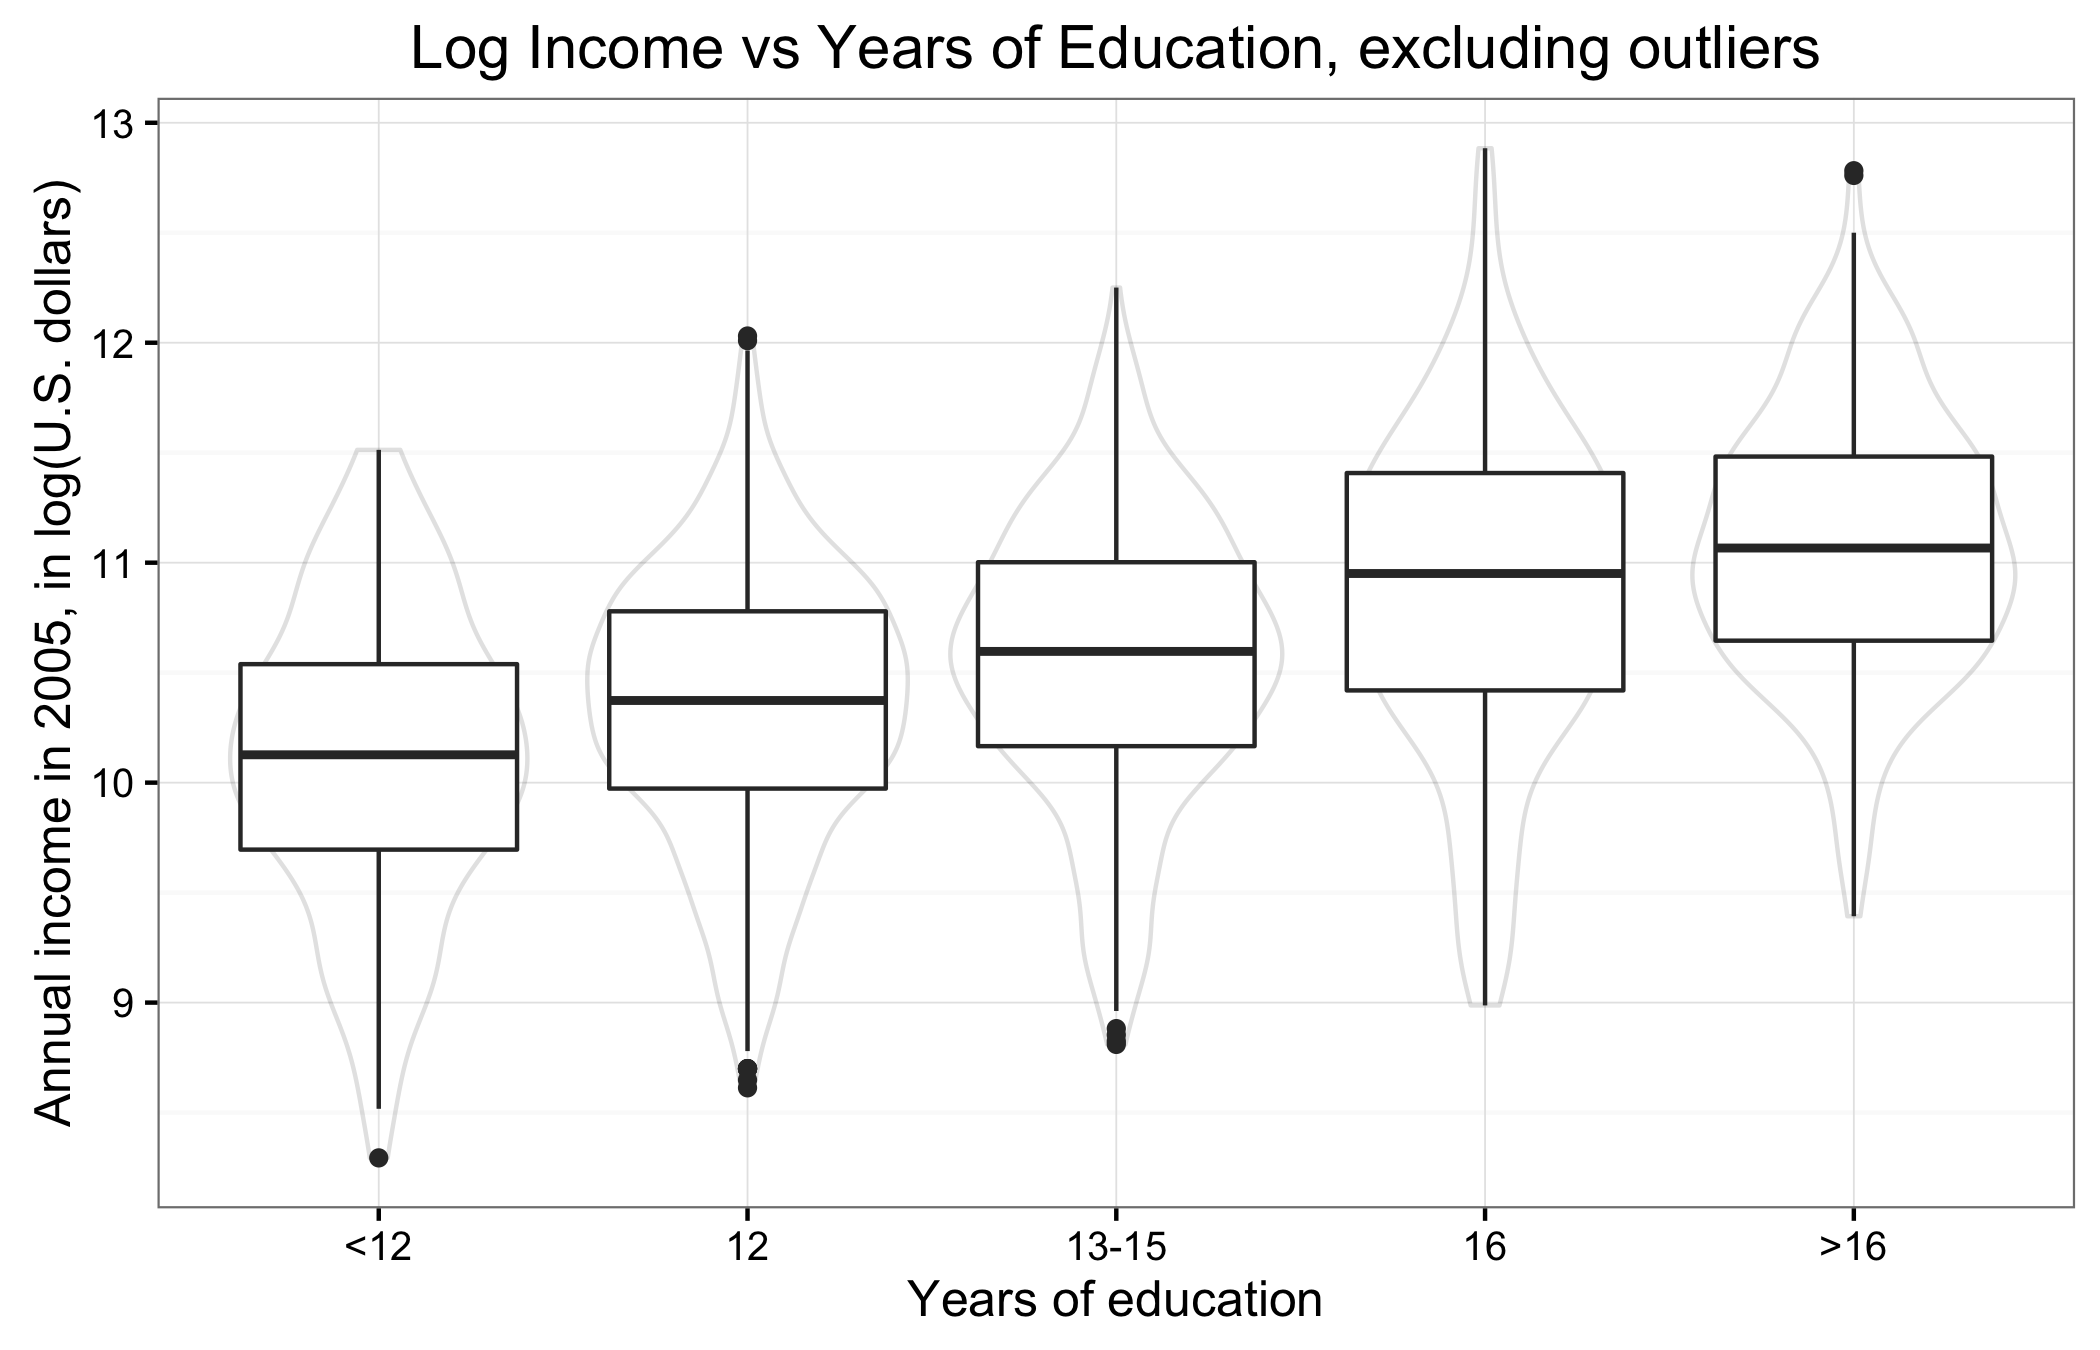
\includegraphics[width=4.25in]{2c.png}
	\caption{Log(Income) vs Years of Education for 2,432 observations (i.e., excluding 152 outliers) among 5 ``Years of Education'' groupings.}
	\label{fig:2c}
\end{figure}



\subpart \textbf{(16) vs (13--15)}

\begin{codeSmall}
> CompareTwoEducGroups(data_frame=incomeEduData, Educ_groups=c("16", "13-15"))
 oneSidedPVal      estimate confInt_lower confInt_upper 
 7.649007e-12  1.500615e+00  1.335230e+00  1.686486e+00 
\end{codeSmall}

The data provides convincing evidence that the 16 YEO population earns a higher income than the 13--15 YOE population (one-sided p-value $7.65 \times 10^{-12}$; two-sample t-test). Income is estimated to be $1.50062$ times greater for the those with 16 YOE compared to those with 13--15 YOE, with a 95\% confidence interval of $1.33523$ to $1.68649$ times (i.e., an estimated 50\% increase; 95\% CI from 34\% to 69\%).


\subpart \textbf{(13--15) vs (12)}

\begin{codeSmall}
> CompareTwoEducGroups(data_frame=incomeEduData, Educ_groups=c("13-15", "12"))
 oneSidedPVal      estimate confInt_lower confInt_upper 
 0.0001140482  1.1782093370  1.0799490482  1.2854099405 
\end{codeSmall}

The data provides convincing evidence that the 13--15 YEO population earns a higher income than the 12 YOE population (one-sided p-value $0.00011$; two-sample t-test). Income is estimated to be $1.17821$ times greater for the those with 13--15 YOE compared to those with 12 YOE, with a 95\% confidence interval of $1.07995$ to $1.28541$ times (i.e., an estimated 17\% increase; 95\% CI from 8.0\% to 29\%).


\subpart \textbf{(12) vs ($<$12)}


\begin{codeSmall}
> CompareTwoEducGroups(data_frame=incomeEduData, Educ_groups=c("12", "<12"))
 oneSidedPVal      estimate confInt_lower confInt_upper 
 0.0000204658  1.3880147741  1.1872749406  1.6226949185 
\end{codeSmall}

The data provides convincing evidence that the 12 YEO population earns a higher income than the $<$12 YOE population (one-sided p-value $0.00002$; two-sample t-test). Income is estimated to be $1.38801$ times greater for the those with 12 YOE compared to those with $<$12 YOE, with a 95\% confidence interval of $1.18727$ to $1.62269$ times (i.e., an estimated 39\% increase; 95\% CI from 19\% to 62\%).

\end{subparts}


\end{parts}


\titledquestion{\ramsey 6.12}

The quantity of interest is the linear combination
$$\gamma=\frac{\mu_{amputee} + \mu_{crutches} + 
\mu_{wheelchair}}{3} - \frac{\mu_{hearing}}{1},$$

which we estimate by

$$g=\frac{\overline{Y}_{amputee} + \overline{Y}_{crutches} + 
\overline{Y}_{wheelchair}}{3} - \frac{\overline{Y}_{hearing}}{1},$$ where the amputee, crutches, and wheelchair groups are handicaps of ``mobility'', and the hearing group is a handicap of ``communication''. Since the coefficients sum to 0, $g$ is a linear contrast.

We're testing whether the average of the mean scores for the mobility group is equal to the mean score of the communication group. That is, $H_0: g=0,\ H_A: g\neq0$.

Using the \texttt{gmodels::fit.contrast} R function, the data provides moderate evidence that the average of the mean scores for the mobility group is not equal to the mean score of the communication group (two-sided p-value 0.02217 for a linear contrast). The score is estimated to be 1.18095 points higher for the mobility group compared to the communication group (95\% confidence interval 0.17452 to 2.18738 points).

\begin{codeSmall}
> # check the order of Handicap factor levels
> levels(handicapData$Handicap)
[1] "Amputee"    "Crutches"   "Hearing"    "None"       "Wheelchair"
> 
> # test if the the avg of score means for
> # amputee/crutches/wheelchair is equal to to hearing
> fit.contrast(model=lm(Score ~ Handicap, data=handicapData),
+              varname="Handicap", coeff=c(1/3, 1/3, -1, 0, 1/3),
+              conf.int=0.95, df=TRUE)
                                      Estimate Std. Error t value   Pr(>|t|) DF lower CI upper CI
Handicap c=( 0.333 0.333 -1 0 0.333 ) 1.180952  0.5039353 2.34346 0.02217534 65 0.174524 2.187381
\end{codeSmall}$



\titledquestion{\ramsey 6.15}

Test scores for the experimental CAD instruction course are shown below:
\begin{figure}[!h]
	\centering
	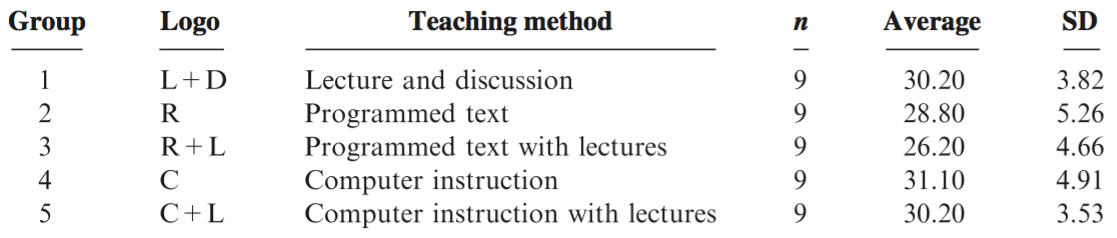
\includegraphics[width=0.8\textwidth]{4.png}
	\label{fig:4}
\end{figure}

\begin{parts}

\part \textit{Compute the pooled estimate of the standard deviation from these summary statistics.}

The pooled estimate of the standard deviation $s_p$ is given by
\begin{align*}
s_p &= \sqrt{\frac{\sum_{i=1}^{5} (n_i -1 ) s_i^2}{\sum_{i=1}^{5} (n_i -1 )}} \\
&= \sqrt{\frac{(9-1)(3.82)^2 + (9-1)(5.26)^2 + (9-1)(4.66)^2 + (9-1)(4.91)^2 + (9-1)(3.53)^2}{(9-1) \cdot 5}} \\
&=4.484297,
\end{align*}

and has $\text{d.f.}=9+9+9+9+9-5=40$ degrees of freedom.


\part \textit{Determine a set of coefficients that will contrast the methods using programmed text as part of the method (groups 2 and 3) with those that do not use programmed text (1, 4, and 5).}

For groups 1 through 5, respectively, the coefficients $C_i$ contrasting groups 2 and 3 with groups 1, 4, and 5 are
$$\left(\frac{1}{3}, -\frac{1}{2}, -\frac{1}{2}, \frac{1}{3}, \frac{1}{3}\right).$$

\part \textit{Estimate the contrast in (b) and compute a 95\% confidence interval.}

An estimate of the linear contrast of interest is
\begin{align*}
g &= \frac{\overline{Y}_{L+D} + \overline{Y}_{C} + 
\overline{Y}_{C+L}}{3} - \frac{\overline{Y}_{R} + \overline{Y}_{R+L}}{2} \\
&= \frac{30.20 + 31.10 + 30.20}{3} - \frac{28.80 + 26.20}{2} \\
&= 3.
\end{align*}

The standard error of the estimate is
\begin{align*}
\text{SE}(g) &= s_p \sqrt{\sum_{i=1}^5\frac{C_i^2}{n_i}} \\
&= (4.484297) \sqrt{  \frac{(1/3)^2}{•9}  +  \frac{(-1/2)^2}{•9}  + \frac{(-1/2)^2}{•9}  + \frac{(1/3)^2}{•9}  + \frac{(1/3)^2}{•9}  } \\
&= 1.364528.
\end{align*}

A 95\% confidence interval is
\begin{gather*}
g \pm t_{40}(0.975) \cdot \text{SE}(g) \\
3 \pm 2.021075 \cdot 1.364528 \\
3 \pm 2.757814 \\
\Rightarrow 0.2421858 \leq g \leq 5.757814.
\end{gather*}


\end{parts}




\titledquestion{\ramsey 6.16}

\textit{A study involving 36 subjects randomly assigned six each to six treatment groups gives an ANOVA F-test with p-value = 0.0850. What multipliers are used to construct 95\% confidence intervals for treatment differences with the following methods:}

\begin{parts}

\part \textbf{LSD}

For the LSD, the multiplier $M$ in the interval half-width is given by the $100(1-\frac{\alpha}{2})$\% critical value in the t-distribution with degrees of freedom equal to those associated with the pooled SD (here, $\text{d.f.}_{s_p} = (6+6+6+6+6+6)-6 = 30$).

Therefore, $M = t_{\text{30}}(1-\frac{0.05}{2}) = t_{30}(0.975) = 2.042272$.

\begin{codeSmall}
> # multiplier for LSD
> qt(p=(1-(0.05/2)), df=30)
[1] 2.042272
\end{codeSmall}


\part \textbf{F-protected LSD}

Since the p-value from the F-test is large ($>$0.05), we can't declare any individual difference significant, and neither the Tuker-Kramer nor the Scheffe multipliers control either the individual or familywise success rate at 95\%.


\part \textbf{Tukey–Kramer}

In the Tukey-Kramer procedure, the multiplier $M$ is given by $[q_{I, (n-I)}(1-\alpha)]/\sqrt{2}$, where $[q_{I, (n-I)}(1-\alpha)]$ is the quantile function of the studentized range distribution with $I$ groups and $(n-I)$ degrees of freedom.

Therefore, $M=[q_{6, (36-I6)}(1-0.05)]/\sqrt{2} = 3.041594$.

\begin{codeSmall}
> # multiplier for Tukey-Kramer
> qtukey(p=(1-0.05), nmeans=6, df=30) / sqrt(2)
[1] 3.041594
\end{codeSmall}


\part \textbf{Bonferroni}

In the Bonferroni procedure, the multiplier $M$ is given by $t_{\text{d.f.}}(1-\frac{\alpha}{2k})$, where $k=\frac{I(I-1)}{2}$ is the number of pairs of means to be compared and d.f. is the degrees of freedom associated with the pooled SD.


Here, $k=\frac{6(6-1)}{2} = 15$, therefore, $M = t_{30}(1-\frac{0.05}{2 \cdot 15}) = t_{30}(0.9983333) = 3.188806$.

\begin{codeSmall}
> # multiplier for Bonferroni
> qt(p=(1-(0.05/(2*15))), df=30)
[1] 3.188806
\end{codeSmall}


\part \textbf{Scheffe}

In the Scheffe procedure, the multiplier $M$ is given by $\sqrt{(I-1)F_{(I-1), \text{d.f.}}(1-\alpha)}$, where $F_{(I-1), \text{d.f.}}(1-\alpha)$ is the $(1-\alpha)$th percentile of the F-distribution with $(I-1)$ and d.f. degrees of freedom.

Therefore $M=\sqrt{(6-1)F_{(6-1), \text{30}}(1-0.05)} = \sqrt{5 \cdot F_{5, \text{30}}(0.95)} = \sqrt{5 \cdot 2.533555} = 3.559181$.

\begin{codeSmall}
> # multiplier for Scheffe
> sqrt(5 * qf(p=(1-0.05), df1=5, df2=30))
[1] 3.559181
\end{codeSmall}


\end{parts}



\titledquestion{\ramsey 6.23}

The data provides moderately strong, but not convincing evidence that there are differences in average weight loss among these diets (a p-value of 0.04086 from a one-way ANOVA F-test). 

The ANOVA table testing for a difference in weight loss after 24 months of dieting is shown below, and a boxplot of these weight losses is shown in Figure \ref{fig:6}.

\begin{center}
  \begin{tabular}{ l c c c c c}
    Source of Variation & Sum of Squares & d.f. & Mean Square & F-Statistic & p-Value \\ \hline \hline
    Between Groups & 216.9 & 2 & 108.430 & 3.2358 & 0.04086 \\
    Within Groups & 9013.9 & 269 & 33.509 & & \\ \hline
    Total & 9230.753 & 271 & & &
  \end{tabular}
\end{center}
\quad \\

\begin{figure}[!h]
	\centering
	\captionsetup{width=0.8\textwidth}
	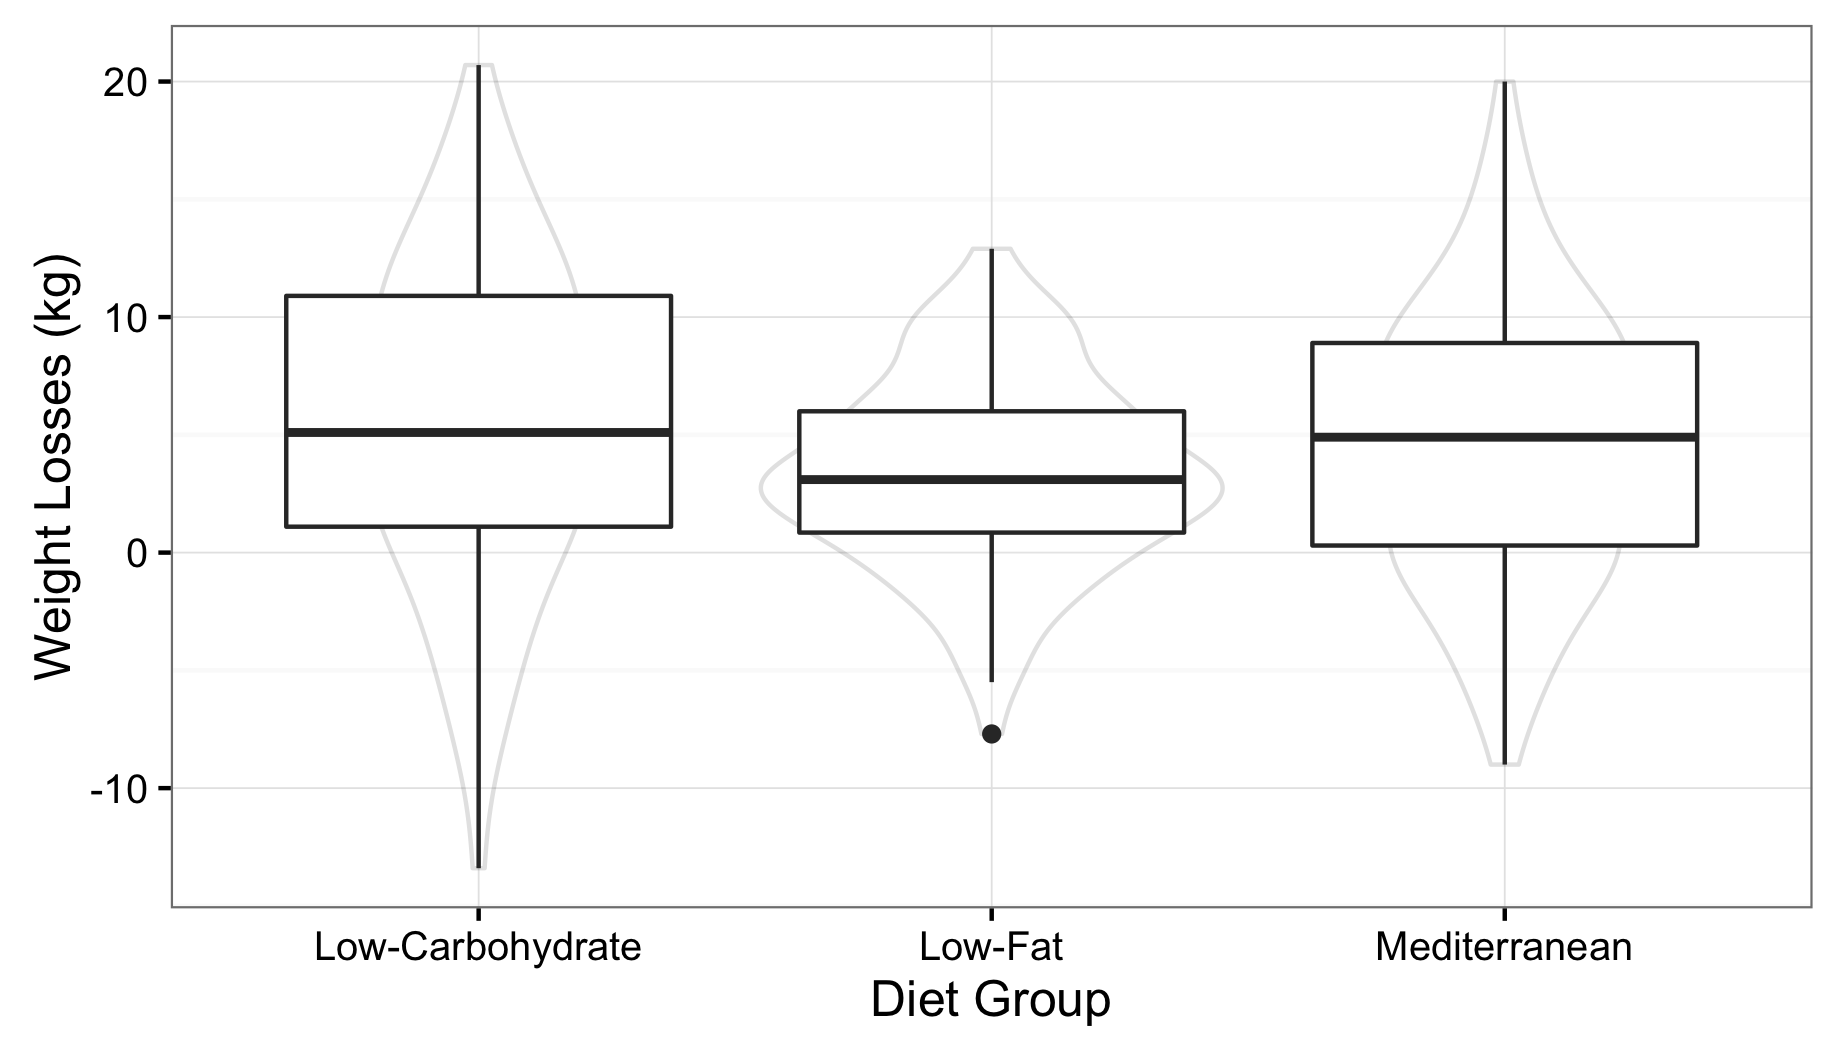
\includegraphics[width=4.25in]{6.png}
	\caption{Weight losses (in kg) of 272 participants who dieted for two years on one of three different diets.}
	\label{fig:6}
\end{figure}

The difference between the average weight loss in the Low-Carbohydrate group and the Low-Fat group is difficult to attribute to chance. The weight loss in the Low-Carbohydrate group is estimated to be 2.1828 kg higher than in the Low-Fat group, with a 95\% confidence interval from 0.1408 to 4.2248 kg based on the Tukey-Kramer procedure.

The difference between the average weight loss in the Mediterranean and Low-Fat groups, and the difference between the average weight loss in the Low-Carbohydrate and Mediterranean groups are not significant.

\begin{codeSmall}
> TukeyHSD(x=aov(lm(WtLoss24 ~ Group, data = dietData)), which="Group",
+ ordered=TRUE, conf.level=0.95)
  Tukey multiple comparisons of means
    95% family-wise confidence level
    factor levels have been ordered

Fit: aov(formula = lm(WtLoss24 ~ Group, data = dietData))

$Group
                                    diff        lwr      upr     p adj
Mediterranean-Low-Fat          1.2978952 -0.6974180 3.293208 0.2771180
Low-Carbohydrate-Low-Fat       2.1828035  0.1408361 4.224771 0.0329364
Low-Carbohydrate-Mediterranean 0.8849083 -1.1622656 2.932082 0.5656813
\end{codeSmall}$



\end{questions}

%\listoftodos

\end{document}